% 第4章 模型求解

\section{模型求解}

\subsection{求解流程说明}

模型求解过程围绕"先识别基准动态，再检验扩展作用"的顺序展开。第一步，从日对数收益率出发构造主因变量和辅助因变量，并进一步生成HAR历史状态变量。第二步，把月度宏观变量按信息可得性原则映射到日频样本。第三步，在训练集上估计HAR\_OLS、HARX\_OLS与HARX-lite\_OLS，并计算HAC稳健标准误和相关统计量。第四步，在相同训练/测试划分下对模型进行样本外评估，以判断基准模型和扩展模型在外推表现上的差异。最后再通过非重叠窗口、单变量宏观扩展和分样本比较完成收尾检验。

这一求解思路与老版本"两阶段收益率—偏离"框架相比更集中。过去的第一阶段承担的是条件预期收益率构造任务，现在的主模型则直接面向"短期不稳定性"这一更可解释的状态指标。这样一来，模型求解不再需要通过高维混频权重去追求微弱的收益率样本外改进，而是转向利用HAR结构识别更稳健的时间尺度效应。

\subsection{主目标\texttt{future\_absret\_5}的HAR基准结果}

HAR\_OLS的估计结果表明，\texttt{past\_absret\_5}的系数为0.8236，HAC标准误为0.0294，\(t\)值达到28.0223；\texttt{past\_absret\_20}的系数为0.1072，\(p\)值为0.0060；\texttt{past\_absret\_60}的系数为0.0100，\(p\)值为0.7446。模型的训练集\(R^2\)为0.7924，调整后\(R^2\)为0.7920，AIC为-13891.86，BIC为-13870.62。Durbin--Watson统计量为1.9254，接近2，但Ljung--Box与ARCH--LM检验均显示残差仍存在序列相关和异方差，因此采用HAC推断是必要的。

这些结果说明，未来一周平均波动幅度的主要解释来源是近5日和近20日的历史不稳定状态，60日尺度在控制其他变量后几乎不再贡献显著解释。换到金融学语言中，这意味着市场不稳定性的延续主要受短期与中期状态驱动，而较长期历史背景对未来一周幅度的边际作用已经很弱。

% 表4-1：future_absret_5的HAR_OLS回归结果
\begin{table*}[htbp]
\centering
\footnotesize
\caption{\texttt{future\_absret\_5}的HAR\_OLS回归结果}
\label{tab:har-ols}
\begin{tabular}{lccccc}
\topline
变量 & 系数 & HAC标准误 & \(t\)值 & \(p\)值 & 95\%置信区间 \\
\midline
\texttt{const} & 0.000506 & 0.000164 & 3.0917 & 0.0020 & [0.000185, 0.000828] \\
\texttt{past\_absret\_5} & 0.823616 & 0.029391 & 28.0223 & 0.0000 & [0.765963, 0.881269] \\
\texttt{past\_absret\_20} & 0.107151 & 0.038919 & 2.7532 & 0.0060 & [0.030809, 0.183493] \\
\texttt{past\_absret\_60} & 0.009980 & 0.030625 & 0.3259 & 0.7446 & [-0.050092, 0.070053] \\
\midline
\multicolumn{6}{l}{模型诊断：\(R^2\)=0.7924，调整后\(R^2\)=0.7920，AIC=-13891.86，BIC=-13870.62，DW=1.9254} \\
\bottomline
\end{tabular}
\end{table*}

\subsection{HARX扩展结果与HARX-lite比较}

在HAR基准之上加入四个宏观变量后，HARX\_OLS的训练集\(R^2\)从0.7924小幅上升到0.7931，调整后\(R^2\)从0.7920上升到0.7922，但四个宏观变量单个均未达到常用显著性标准。\texttt{epu\_log\_m1}的系数为-0.000137，\(p\)值0.3967；\texttt{fx\_ret1\_m1}的系数为-0.000654，\(p\)值0.9084；\texttt{ppi\_yoy\_m1}的系数为-0.000024，\(p\)值0.1987；\texttt{m2\_delta1\_m1}的系数为0.000176，\(p\)值0.1632。模型条件数升至4217.07，虽未出现明显共线性爆炸，但数值稳定性较HAR基准更弱。

HARX-lite只保留\texttt{fx\_ret1\_m1}与\texttt{ppi\_yoy\_m1}两个相对更具经济含义的变量，其结果与完整HARX基本相当。训练集\(R^2\)为0.7927，调整后\(R^2\)为0.7920，AIC和BIC略优于完整HARX，但扩展变量仍未显著。这样的结果说明，宏观变量即使经过精简，其增量作用仍然有限，更适合作为补充分析，而不宜替代基准HAR结构。

% 表4-2：future_absret_5的HARX_OLS回归结果
\begin{table*}[htbp]
\centering
\footnotesize
\caption{\texttt{future\_absret\_5}的HARX\_OLS回归结果}
\label{tab:harx-ols}
\begin{tabular}{lccccc}
\topline
变量 & 系数 & HAC标准误 & \(t\)值 & \(p\)值 & 95\%置信区间 \\
\midline
\texttt{const} & 0.001562 & 0.000995 & 1.5705 & 0.1165 & [-0.000389, 0.003513] \\
\texttt{past\_absret\_5} & 0.822169 & 0.028853 & 28.4956 & 0.0000 & [0.765573, 0.878765] \\
\texttt{past\_absret\_20} & 0.108830 & 0.039023 & 2.7889 & 0.0054 & [0.032285, 0.185376] \\
\texttt{past\_absret\_60} & -0.008517 & 0.032633 & -0.2610 & 0.7941 & [-0.072528, 0.055494] \\
\texttt{epu\_log\_m1} & -0.000137 & 0.000162 & -0.8478 & 0.3967 & [-0.000455, 0.000180] \\
\texttt{fx\_ret1\_m1} & -0.000654 & 0.005684 & -0.1150 & 0.9084 & [-0.011804, 0.010496] \\
\texttt{ppi\_yoy\_m1} & -0.000024 & 0.000018 & -1.2859 & 0.1987 & [-0.000059, 0.000012] \\
\texttt{m2\_delta1\_m1} & 0.000176 & 0.000126 & 1.3950 & 0.1632 & [-0.000072, 0.000424] \\
\bottomline
\end{tabular}
\end{table*}

% 表4-3：future_absret_5的HARX-lite回归结果
\begin{table*}[htbp]
\centering
\footnotesize
\caption{\texttt{future\_absret\_5}的HARX-lite回归结果}
\label{tab:harx-lite}
\begin{tabular}{lccccc}
\topline
变量 & 系数 & HAC标准误 & \(t\)值 & \(p\)值 & 95\%置信区间 \\
\midline
\texttt{const} & 0.000655 & 0.000194 & 3.3836 & 0.0007 & [0.000275, 0.001035] \\
\texttt{past\_absret\_5} & 0.822950 & 0.028899 & 28.4767 & 0.0000 & [0.766262, 0.879637] \\
\texttt{past\_absret\_20} & 0.108117 & 0.038904 & 2.7791 & 0.0055 & [0.031804, 0.184429] \\
\texttt{past\_absret\_60} & -0.003404 & 0.032676 & -0.1042 & 0.9170 & [-0.067500, 0.060691] \\
\texttt{fx\_ret1\_m1} & 0.000923 & 0.005641 & 0.1636 & 0.8701 & [-0.010141, 0.011987] \\
\texttt{ppi\_yoy\_m1} & -0.000021 & 0.000018 & -1.1685 & 0.2428 & [-0.000057, 0.000014] \\
\bottomline
\end{tabular}
\end{table*}

\subsection{增量检验与共线性诊断}

HAR与HARX的嵌套检验显示，宏观变量作为一组并未形成稳健的增量解释力。对于\texttt{future\_absret\_5}，加入四个宏观变量后，\(R^2\)仅增加0.000689，调整后\(R^2\)仅增加0.000132，联合F检验统计量为1.2365，对应\(p\)值为0.2934。换言之，尽管扩展模型在训练样本中有极小幅度的拟合提升，但从统计检验意义上看，这种提升不足以支持"宏观变量整体上显著改善解释力"的表述。

共线性诊断方面，HARX\_OLS中的VIF最大值为4.09，HARX-lite中最大值为4.07，均低于5，说明正式模型已不存在前期高维特征设计中的明显共线性问题。宏观变量作用较弱，主要不是由严重多重共线性所致，而更可能源于它们对短期不稳定性的边际解释本身有限。

% 表4-4：主模型样本内外比较
\begin{table*}[htbp]
\centering
\footnotesize
\caption{主模型样本内外比较}
\label{tab:model-comparison}
\begin{tabular}{lcccccc}
\topline
模型 & 训练集\(R^2\) & 调整后\(R^2\) & 测试集\(R^2_{OS}\) & RMSE & MAE & AIC \\
\midline
HAR\_OLS & 0.7924 & 0.7920 & 0.8233 & 0.002109 & 0.001363 & -13891.86 \\
HARX\_OLS & 0.7931 & 0.7922 & 0.8217 & 0.002119 & 0.001374 & -13888.82 \\
HARX\_lite\_OLS & 0.7927 & 0.7920 & 0.8219 & 0.002117 & 0.001375 & -13889.60 \\
HAR\_Ridge & 0.7884 & 0.7880 & 0.8078 & 0.002200 & 0.001410 & -- \\
HARX\_Ridge & 0.7891 & 0.7881 & 0.8061 & 0.002210 & 0.001424 & -- \\
Mean\_Benchmark & -- & -- & 0.0000 & 0.005018 & 0.003247 & -- \\
\bottomline
\end{tabular}
\end{table*}

% 表4-5：HAR与HARX的增量检验结果
\begin{table*}[htbp]
\centering
\footnotesize
\caption{HAR与HARX的增量检验结果}
\label{tab:incremental-tests}
\begin{tabular}{lcccccc}
\topline
目标变量 & 基准模型 & 扩展模型 & \(\Delta R^2\) & \(\Delta\)调整后\(R^2\) & F统计量 & \(p\)值 \\
\midline
\texttt{future\_absret\_5} & HAR\_OLS & HARX\_OLS & 0.000689 & 0.000132 & 1.2365 & 0.2934 \\
\texttt{future\_logrv\_20} & HAR\_OLS & HARX\_OLS & 0.000048 & -0.000018 & 0.7242 & 0.5754 \\
\bottomline
\end{tabular}
\end{table*}

% 表4-6：HARX模型的VIF诊断
\begin{table*}[htbp]
\centering
\footnotesize
\caption{HARX模型的VIF诊断}
\label{tab:vif}
\begin{tabular}{llc}
\topline
模型 & 变量 & VIF \\
\midline
\multirow{7}{*}{HARX\_OLS}
& \texttt{past\_absret\_5} & 2.25 \\
& \texttt{past\_absret\_20} & 4.09 \\
& \texttt{past\_absret\_60} & 3.01 \\
& \texttt{epu\_log\_m1} & 1.02 \\
& \texttt{fx\_ret1\_m1} & 1.06 \\
& \texttt{ppi\_yoy\_m1} & 1.36 \\
& \texttt{m2\_delta1\_m1} & 1.05 \\
\bottomline
\end{tabular}
\end{table*}

% 图4-1：future_absret_5的拟合散点图
\begin{figure}[htbp]
\centering
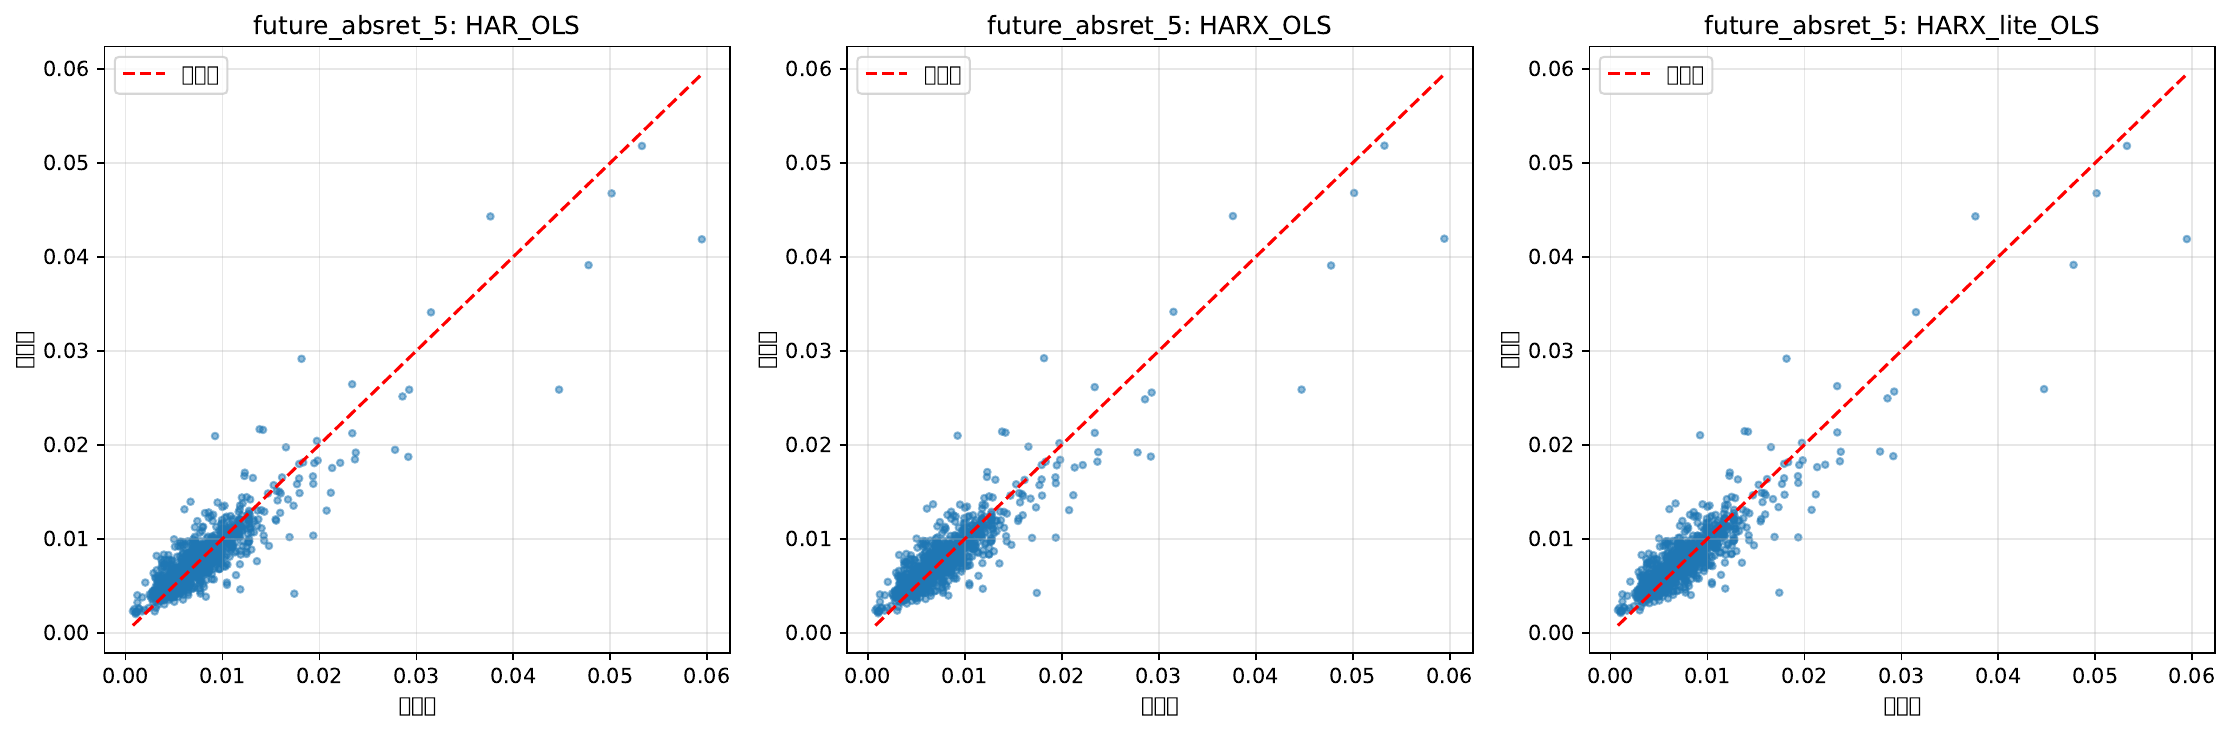
\includegraphics[width=0.85\textwidth]{figures/har_scatter.png}
\caption{\texttt{future\_absret\_5}的HAR\_OLS拟合散点图}
\label{fig:har-fit}
\end{figure}
